\documentclass{article}
\usepackage{amsmath}
\usepackage[mathletters]{ucs}
\usepackage[utf8x]{inputenc}
\usepackage[margin=1.5in]{geometry}
\usepackage{enumerate}
\newtheorem{theorem}{Theorem}
\usepackage{listings} %for kode/lstlisting
\usepackage[dvipsnames]{xcolor}
\usepackage{pgfplots}
\setlength{\parindent}{0cm}
\usepackage{graphics}
\usepackage{graphicx} % Required for including images
\usepackage{subcaption}
\usepackage{bigintcalc}
\usepackage{pythonhighlight} %for pythonkode \begin{python}   \end{python}
\usepackage{appendix}
\usepackage{arydshln}
\usepackage{physics}
\usepackage{tikz-cd}
\usepackage{booktabs} 
\usepackage{adjustbox}
\usepackage{mdframed}
\usepackage{relsize}
\usepackage{physics}
\usepackage[thinc]{esdiff}
\usepackage{fixltx2e}
\usepackage{esint}  %for lukket-linje-integral
\usepackage{xfrac} %for sfrac
\usepackage{hyperref} %for linker, må ha med hypersetup
\usepackage[noabbrev, nameinlink]{cleveref} % to be loaded after hyperref
\usepackage{amssymb} %\mathbb{R} for reelle tall, \mathcal{B} for "matte"-font
\usepackage{verbatim}
\usepackage{graphicx,wrapfig,lipsum,caption} %for wrapping av bilder
\usepackage{mathtools} %for \abs{x}
\usepackage[norsk]{babel}
\definecolor{codegreen}{rgb}{0,0.6,0}
\definecolor{codegray}{rgb}{0.5,0.5,0.5}
\definecolor{codepurple}{rgb}{0.58,0,0.82}
\definecolor{backcolour}{rgb}{0.95,0.95,0.92}
\lstdefinestyle{mystyle}{
    backgroundcolor=\color{backcolour},   
    commentstyle=\color{codegreen},
    keywordstyle=\color{magenta},
    numberstyle=\tiny\color{codegray},
    stringstyle=\color{codepurple},
    basicstyle=\ttfamily\footnotesize,
    breakatwhitespace=false,         
    breaklines=true,                 
    captionpos=b,                    
    keepspaces=true,                 
    numbers=left,                    
    numbersep=5pt,                  
    showspaces=false,                
    showstringspaces=false,
    showtabs=false,                  
    tabsize=2
}

\lstset{style=mystyle}
\author{Oskar Idland}
\title{FYS2130 - Regneoppgaver uke 5}
\date{}
\begin{document}
\maketitle
\newpage

\section*{Til Info}
  Denne obligen er helt avhengig av korrekt kode for å fungere. Koden vedlagt inneholder feil jeg ikke har klart å rett på i tide. Er enkelte av konstantene i STFT som mest sannsynlig er beregnet feil, og for å klare å danne noen form for analyse er trolig noe av beregningene gjort litt feil de også. Resultat matrisen er transponert for å passe med frekvens og sample axene, men er helt tydelig feil når strekene er vertikale istedet for horisontale. Dette er kommentert underveis. Setter pris på tilbakemelding om du ser hva som er feil :)

\section*{Oppgave 1}
\subsection*{a)}
\begin{figure}[h!]
  \centering
  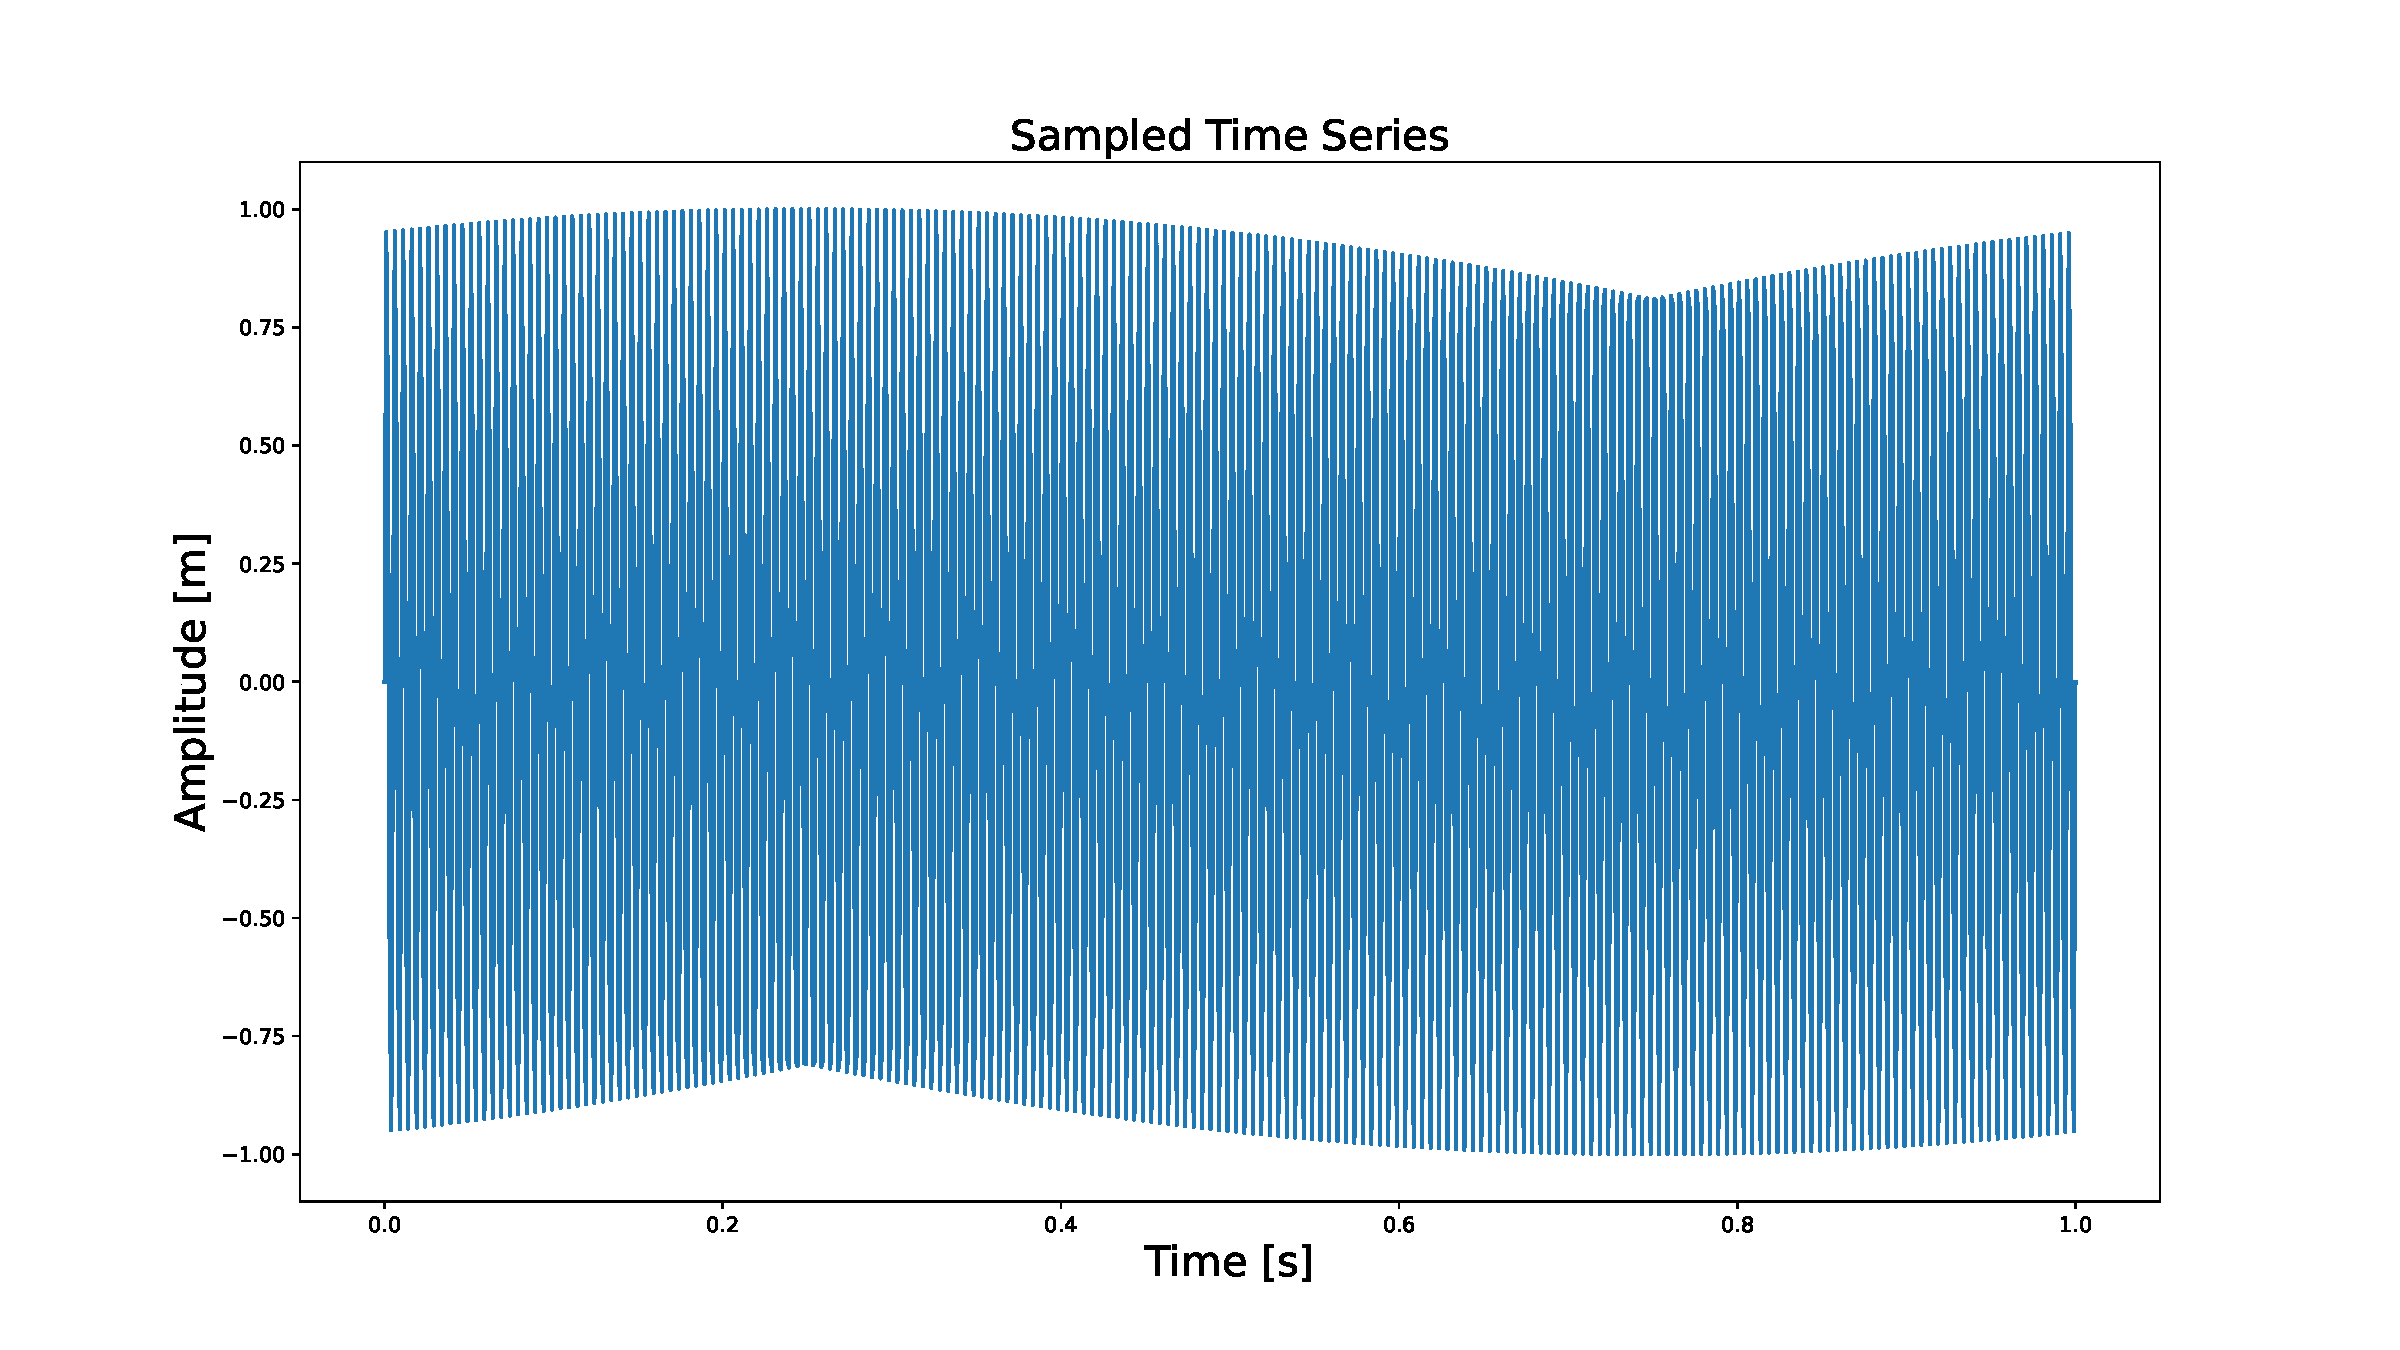
\includegraphics[width = \textwidth]{fig/1.a.1.pdf}
  \caption{Samplet signal}
  \label{fig: 1.a.1}
\end{figure}
\begin{figure}[h!]
  \centering
  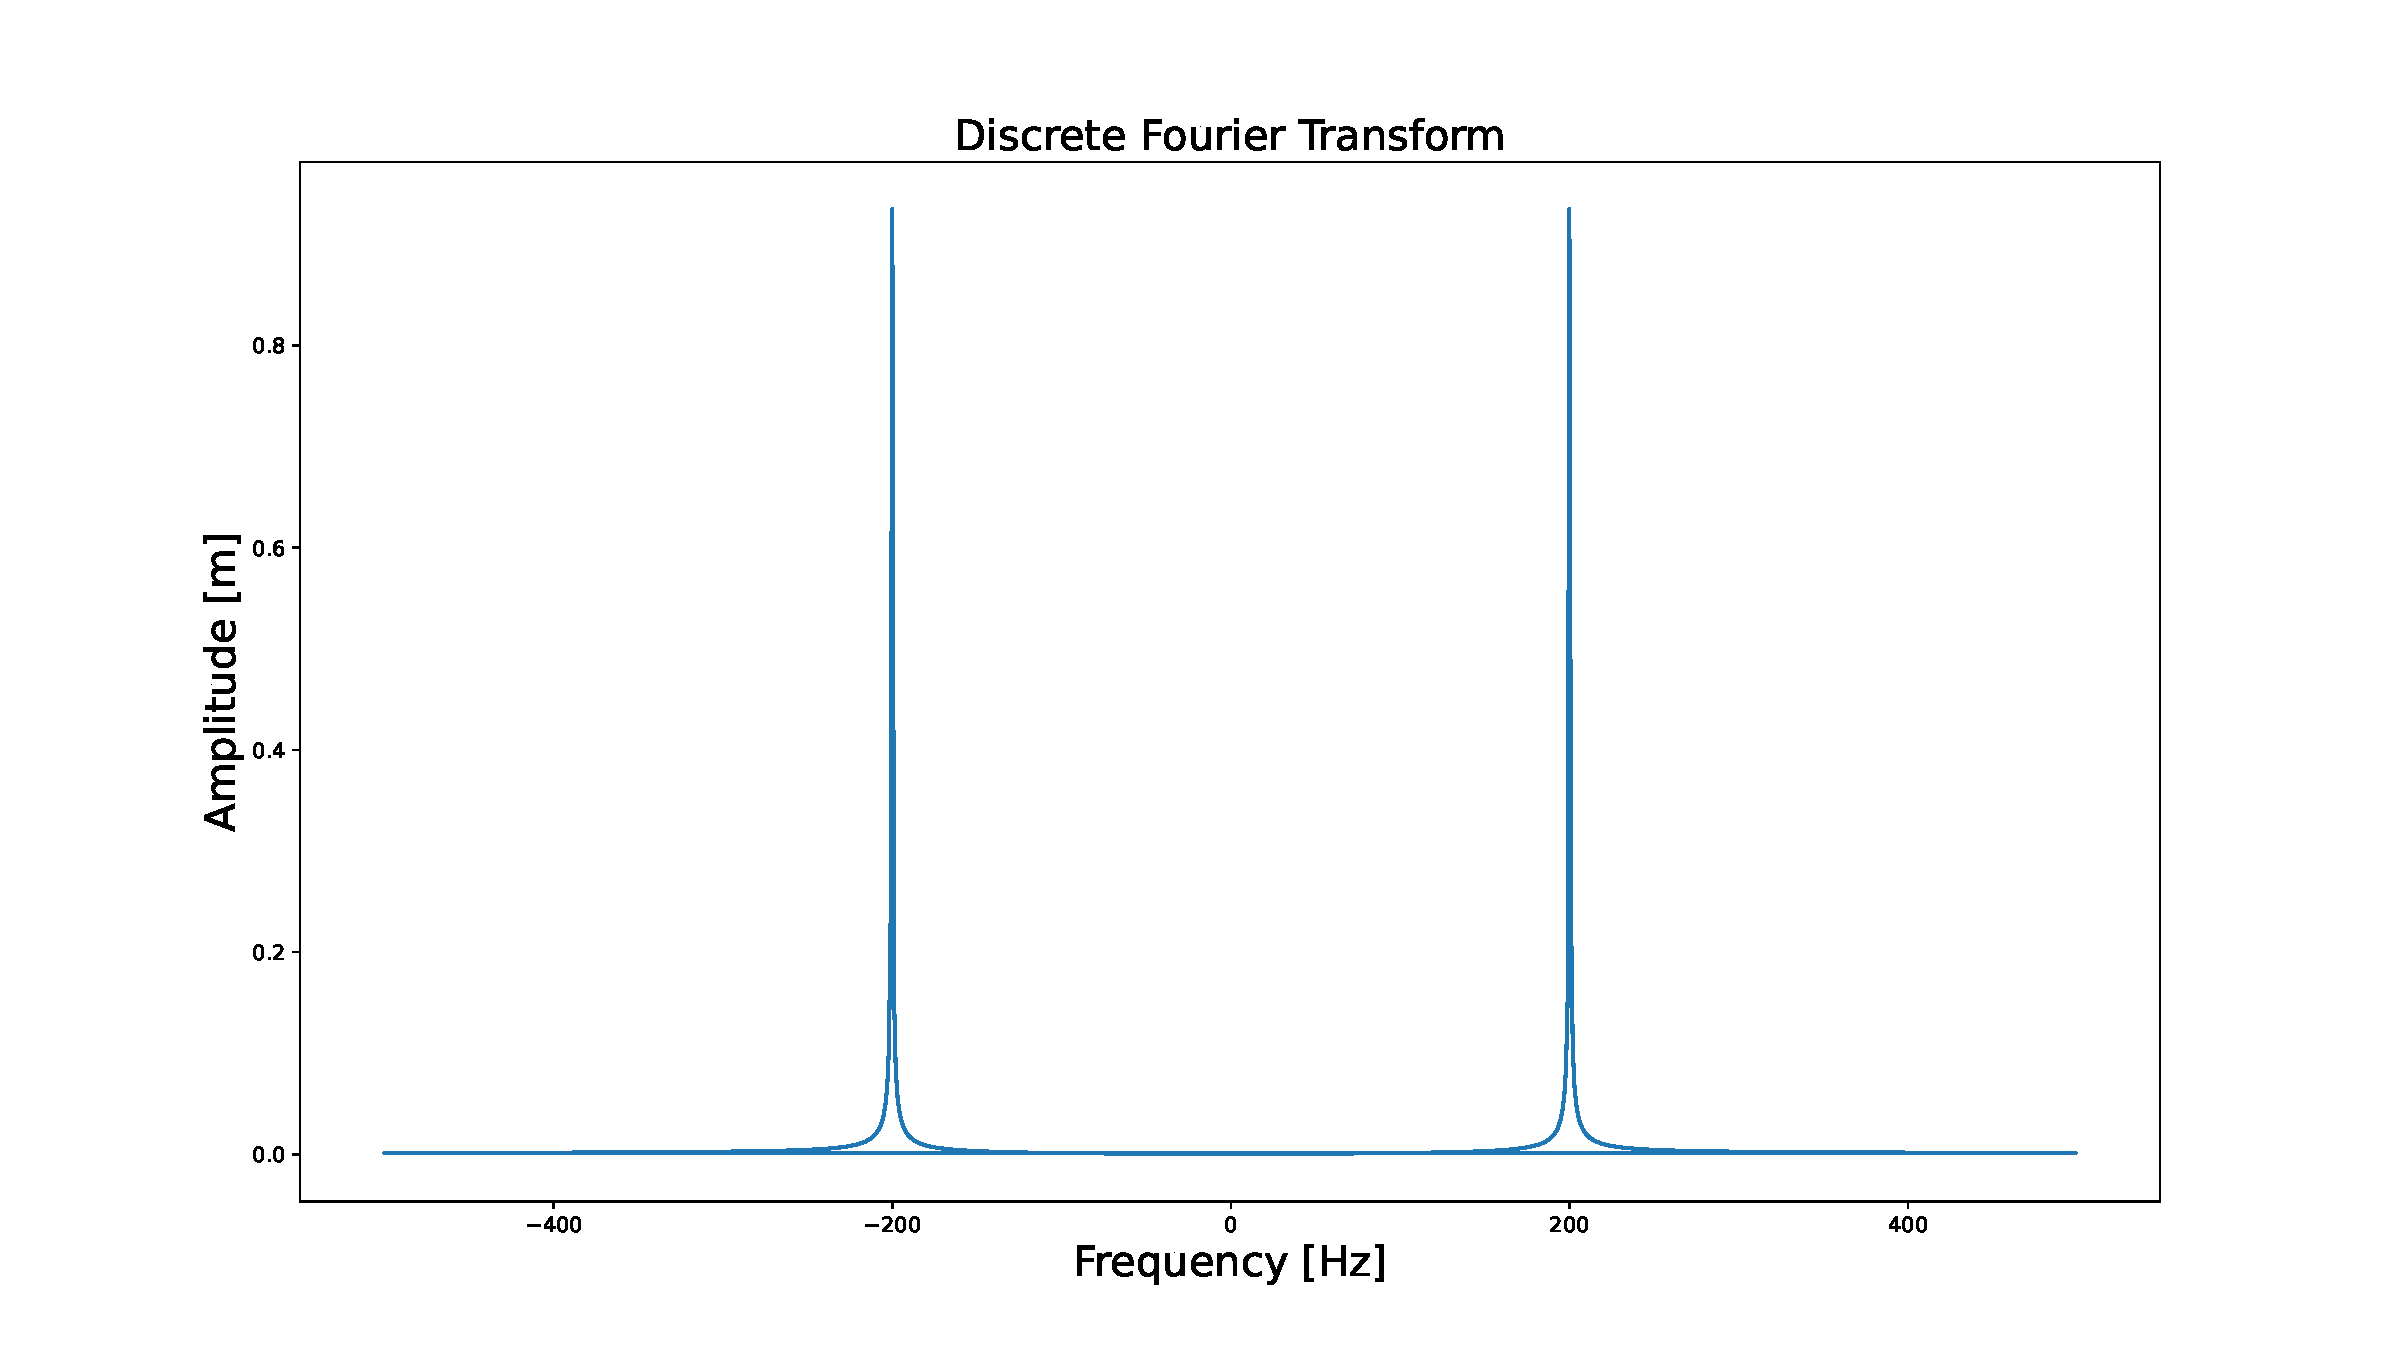
\includegraphics[width = \textwidth]{fig/1.a.2.pdf}
  \caption{Fourier transformasjon}
  \label{fig: 1.a.2}
\end{figure}
Vi ser naturligvis bare på de positive frekvensene. En amplitude på litt under 1 gir mening ettersom integralet under kurven skal være 1 og den har såpass spiss topp. 
% TODO: Dobbelt sjekk

\subsection*{b)}
\begin{figure}[h!]
  \centering
  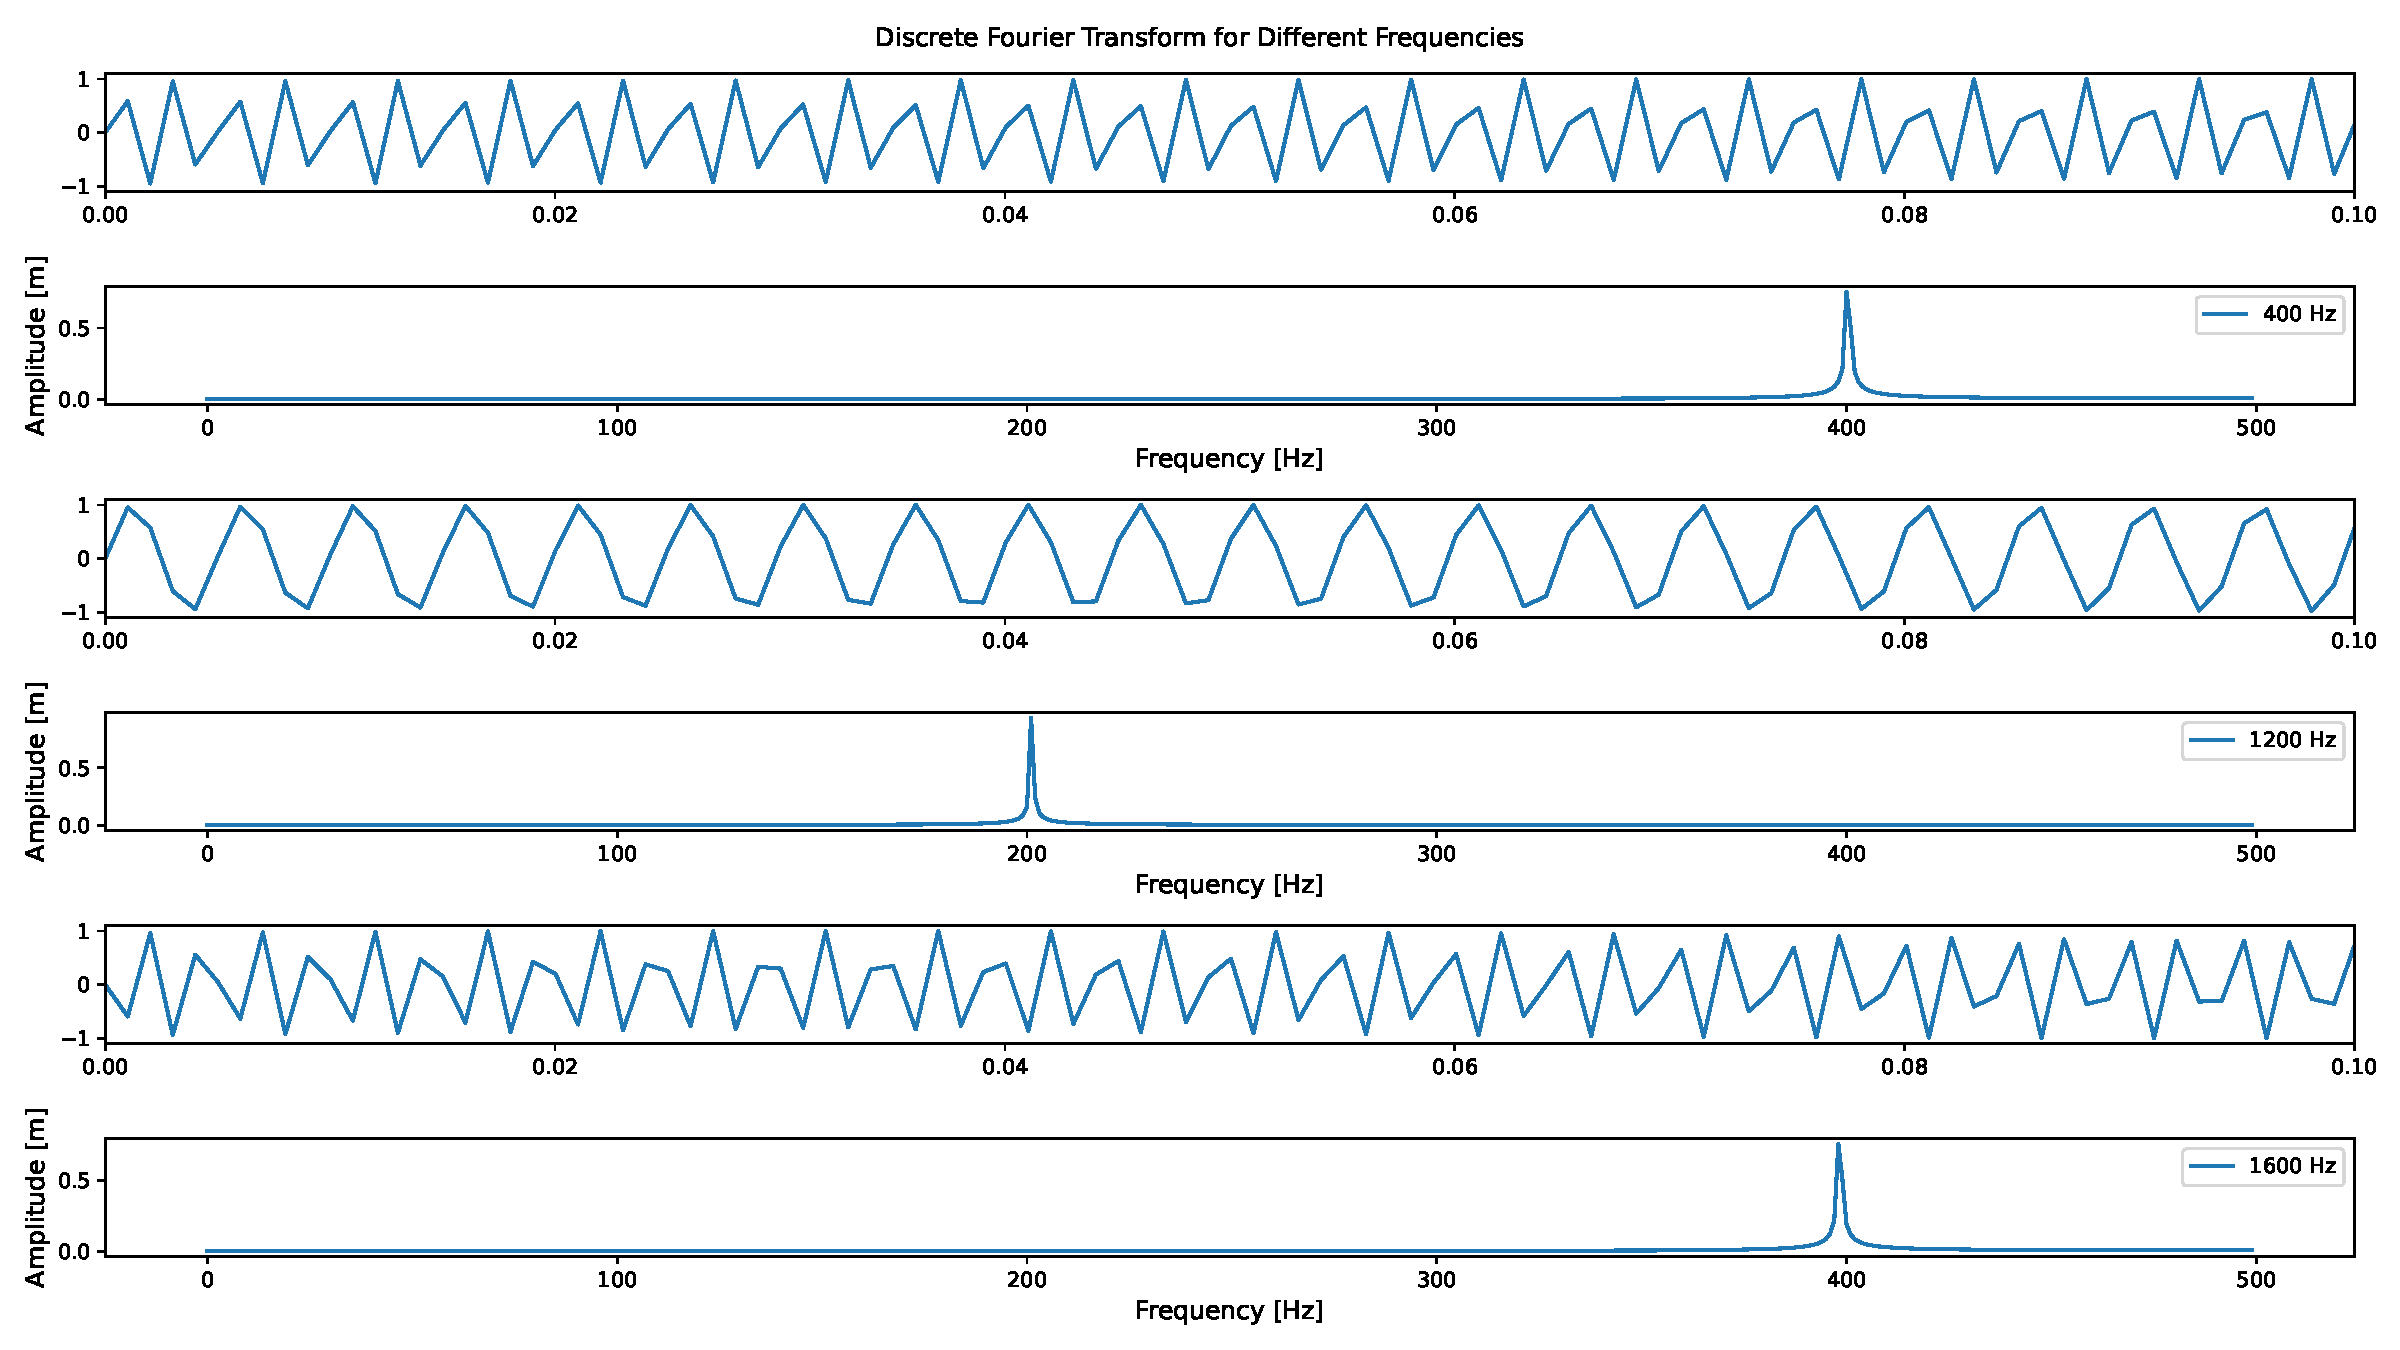
\includegraphics[width = \textwidth]{fig/1.b.pdf}
  \caption{Fourier transformasjon}
  \label{fig: 1.b}
\end{figure}
Nyquist frekvensen er gitt ved vår sampling frekvens $f_s$ og er dermed $f_s / 2 = 5$
kHz. Om denne vil vi ha en speiling vi må se bort ifra. Nyquist frekvensen setter en øvre grense for frekvensene vi kan måle, ettersom vi ikke kan stole på om en frekvens over denne er en del av signalet eller bare en speiling. Det er bare signalet på $400$ Hz som oppfyller dette kravet og er dermed det eneste vi kan stole på. Aliasing oppstår når vi vi under-sampler et signal med en $f_s$ som er mindre en Nyquist frekvensen. Då får vi to frekvenser som er speilinger av hverandre og som dermed ikke kan skilles fra hverandre. Dette ser vi hos på 1200 Hz og 1600 Hz, der Nyquist frekvensen er 600 Hz, og 800 Hz. Dette er ikke med i plottet, men det dukker opp to ekstra topper speilet om disse frekvensene. Ellers vil folding uansett oppstå rundt Nyquist frekvensen, men hvis vi vet ca hvilken frekvens vi leter etter kan vi se bort ifra den. 

\section*{Oppgave 2}
\subsection*{a)}
\begin{figure}[h!]
  \centering
  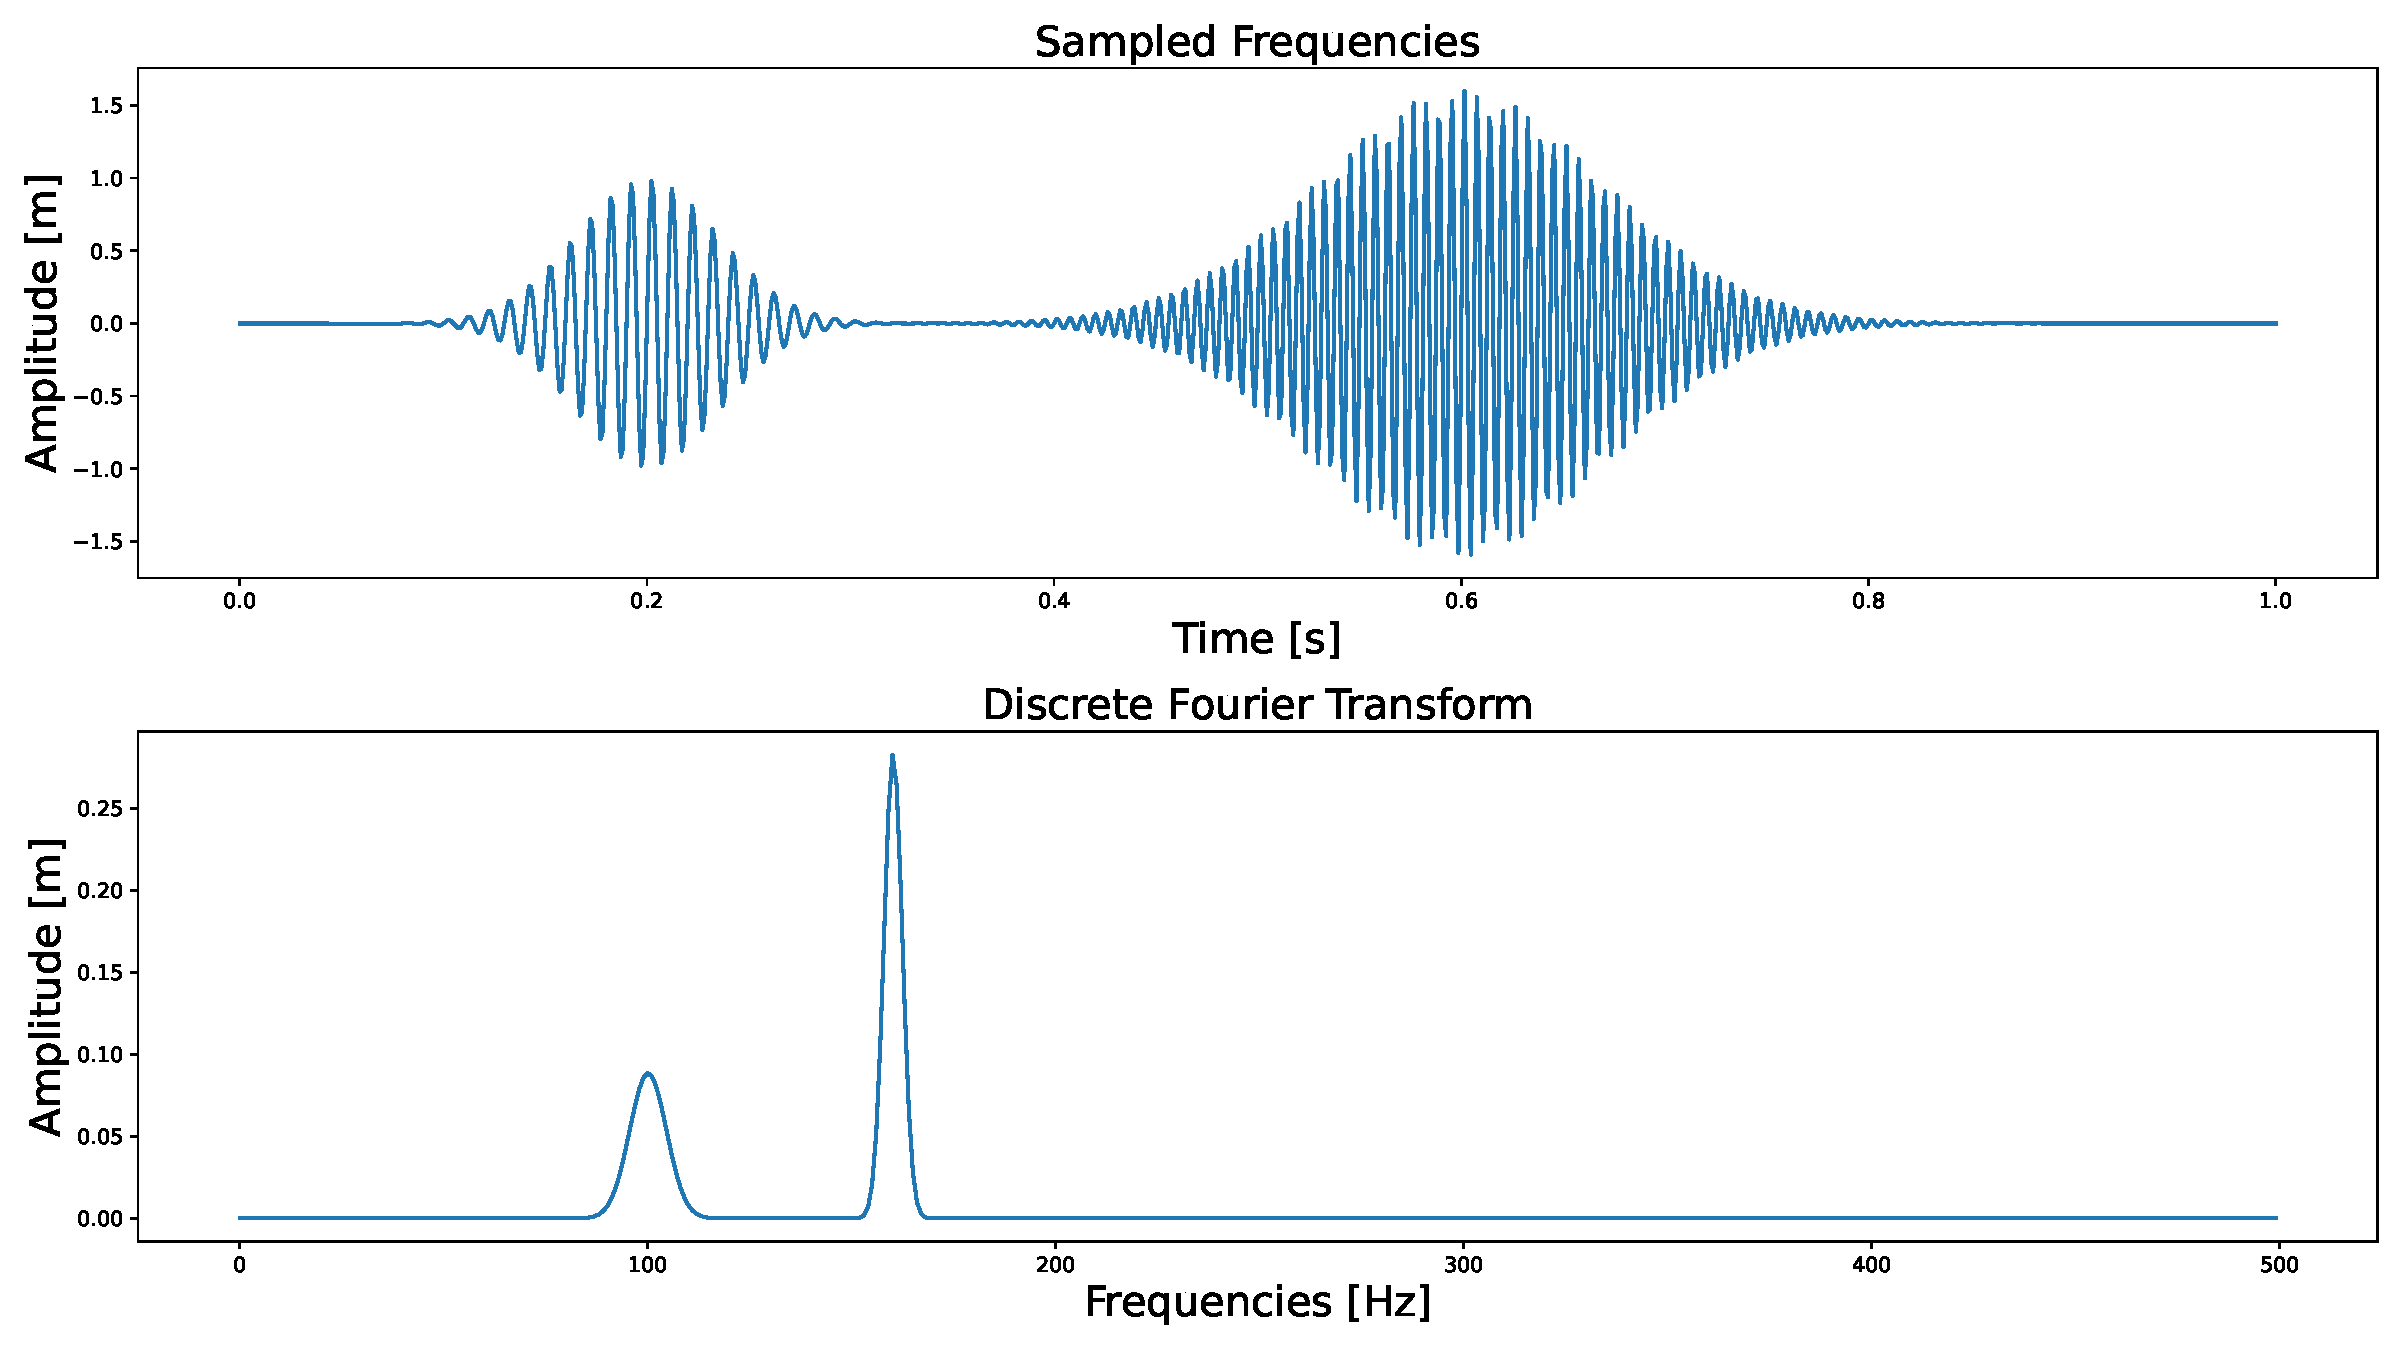
\includegraphics[width = \textwidth]{fig/2.a.pdf}
  \caption{Plot av samplet signal og Fourier transformasjon}
  \label{fig: 2.a}
\end{figure}
\subsection*{b)}
Se vedlagt kode. 
% \lstinputlisting[language=Python, firstline=25, lastline=65]{Oblig_3_kode.py}

\subsection*{c)}
\begin{figure}[h!]
  \centering
  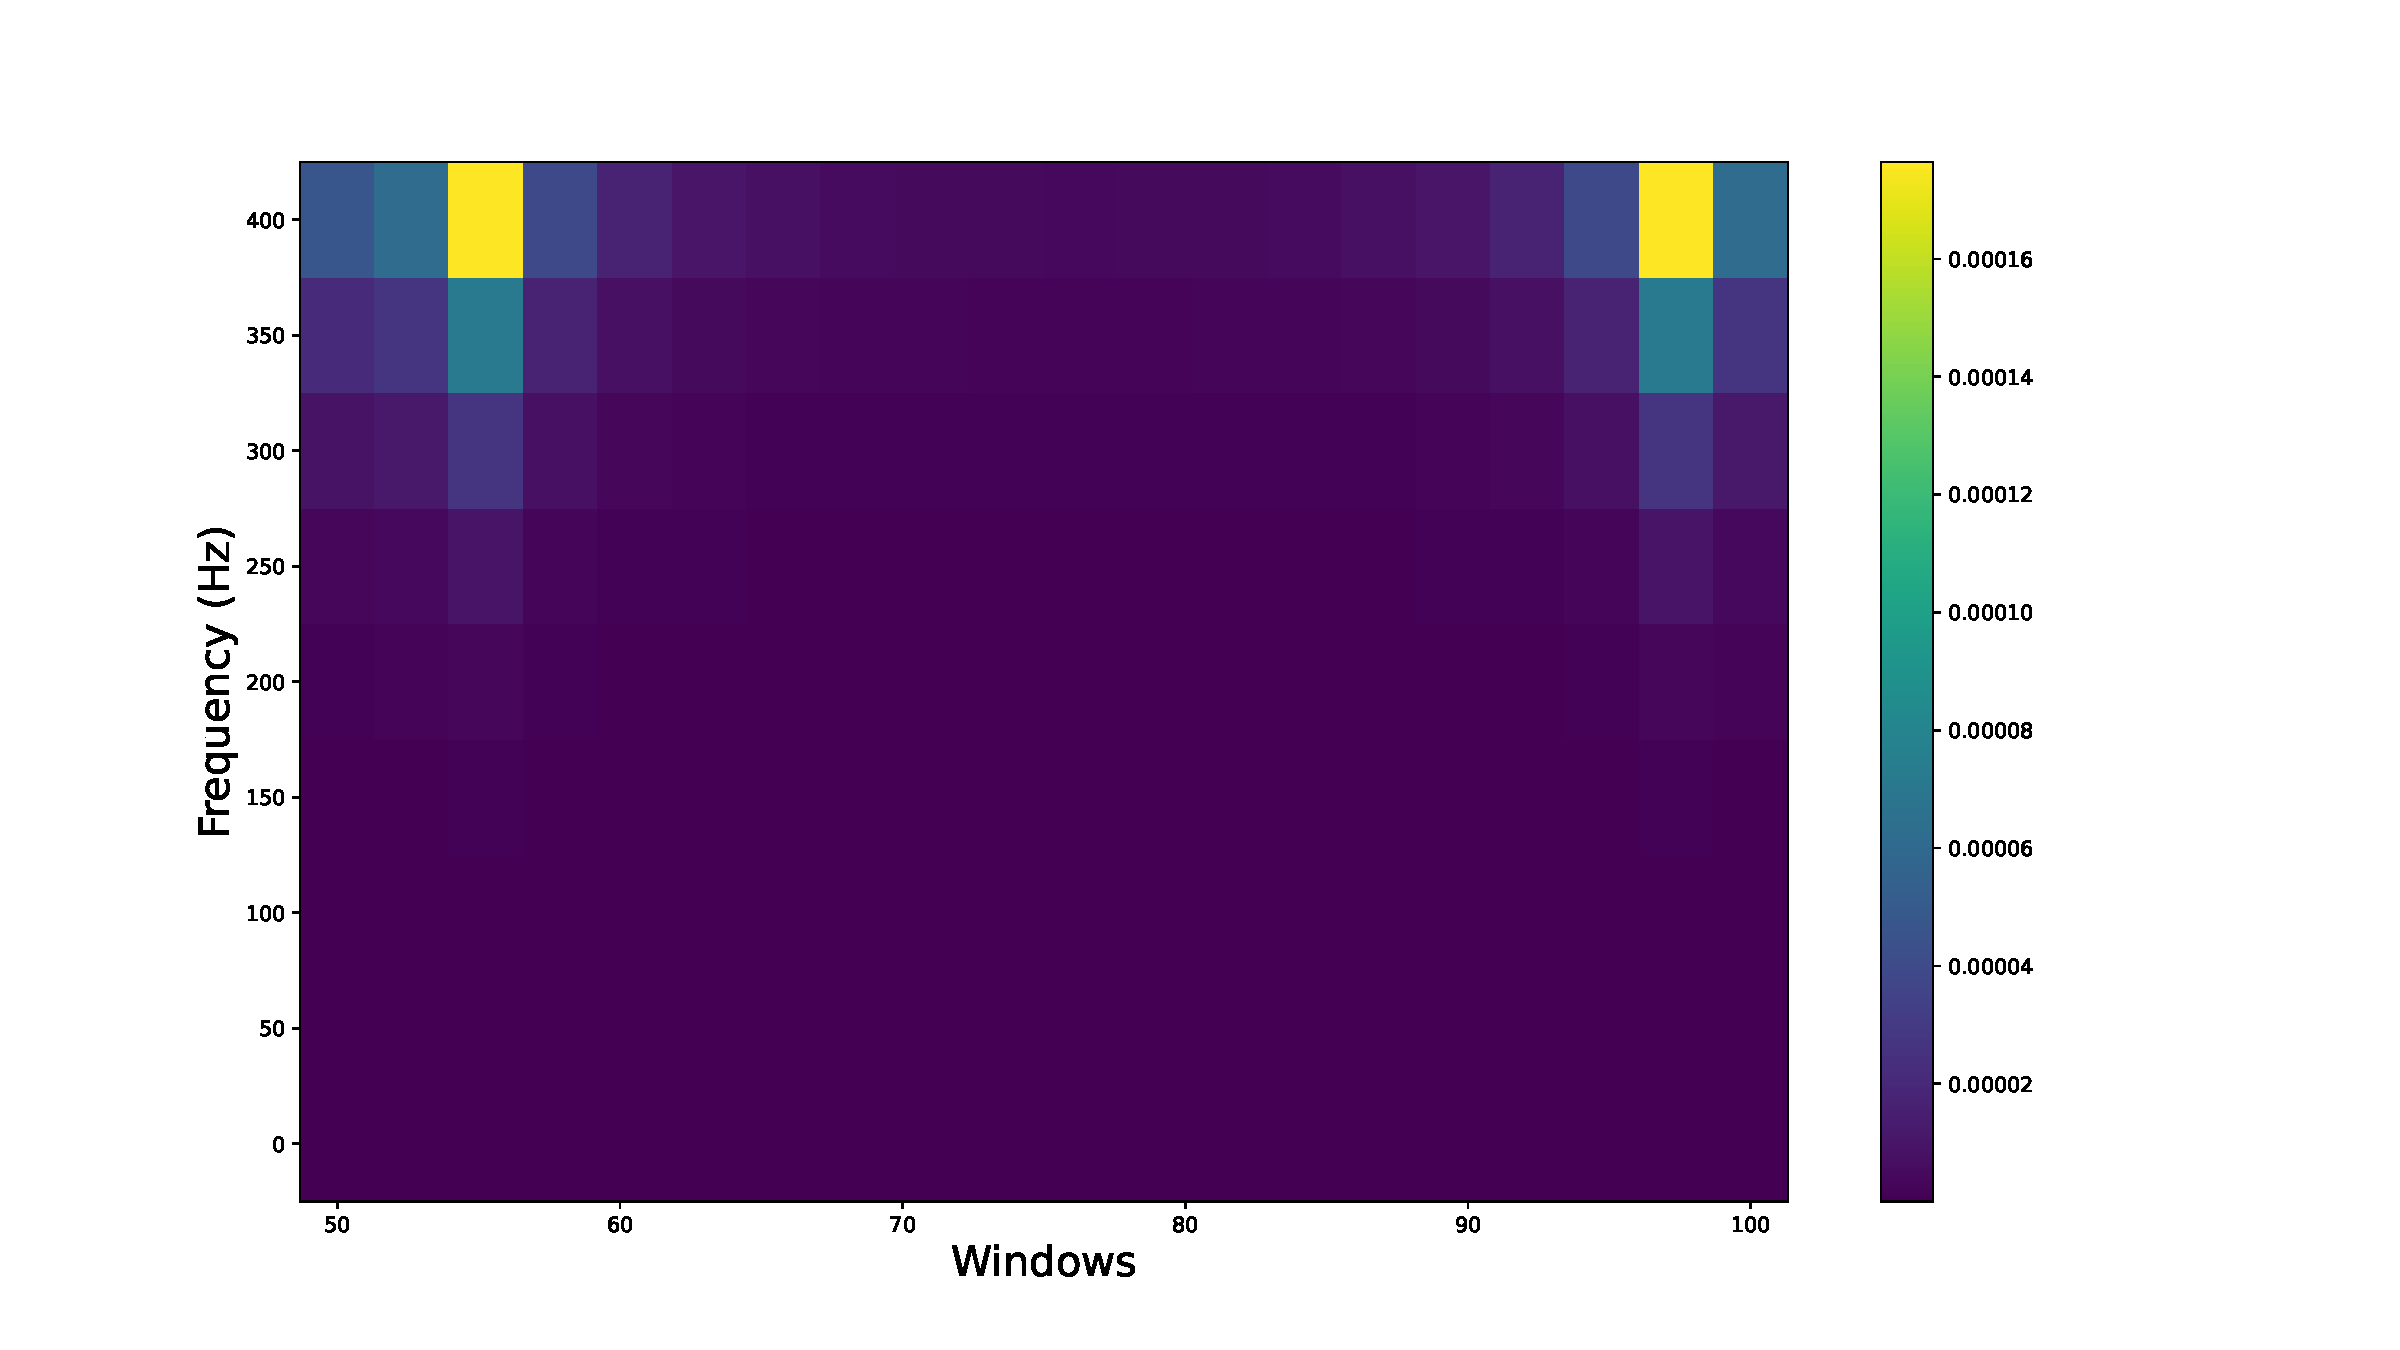
\includegraphics[width = \textwidth]{fig/2.c.1.pdf}
  \caption{Spektrogram ved bruk av egen STFT med tidsvindu på 0.2 sekunder}
  \label{fig: 2.c.1}
\end{figure}

\begin{figure}[h!]
  \centering
  \includegraphics[width = \textwidth]{fig/2.c.2.pdf}
  \caption{Spektrogram ved bruk av egen STFT med tidsvindu på 0.15 sekunder}
  \label{fig: 2.c.2}
\end{figure}
Oppløsning i tid og frekvens har et invers forhold til hverandre så en må velge hva en vil ha fokus på. Med større vinduer får vi dårligere evne til å lese flere frekvenser, men et mindre vindu gjør det også vanskeligere å lese av resultatene.  % TODO: Dobbelt sjekk


\subsection*{d)}
\begin{figure}[h!]
  \centering
  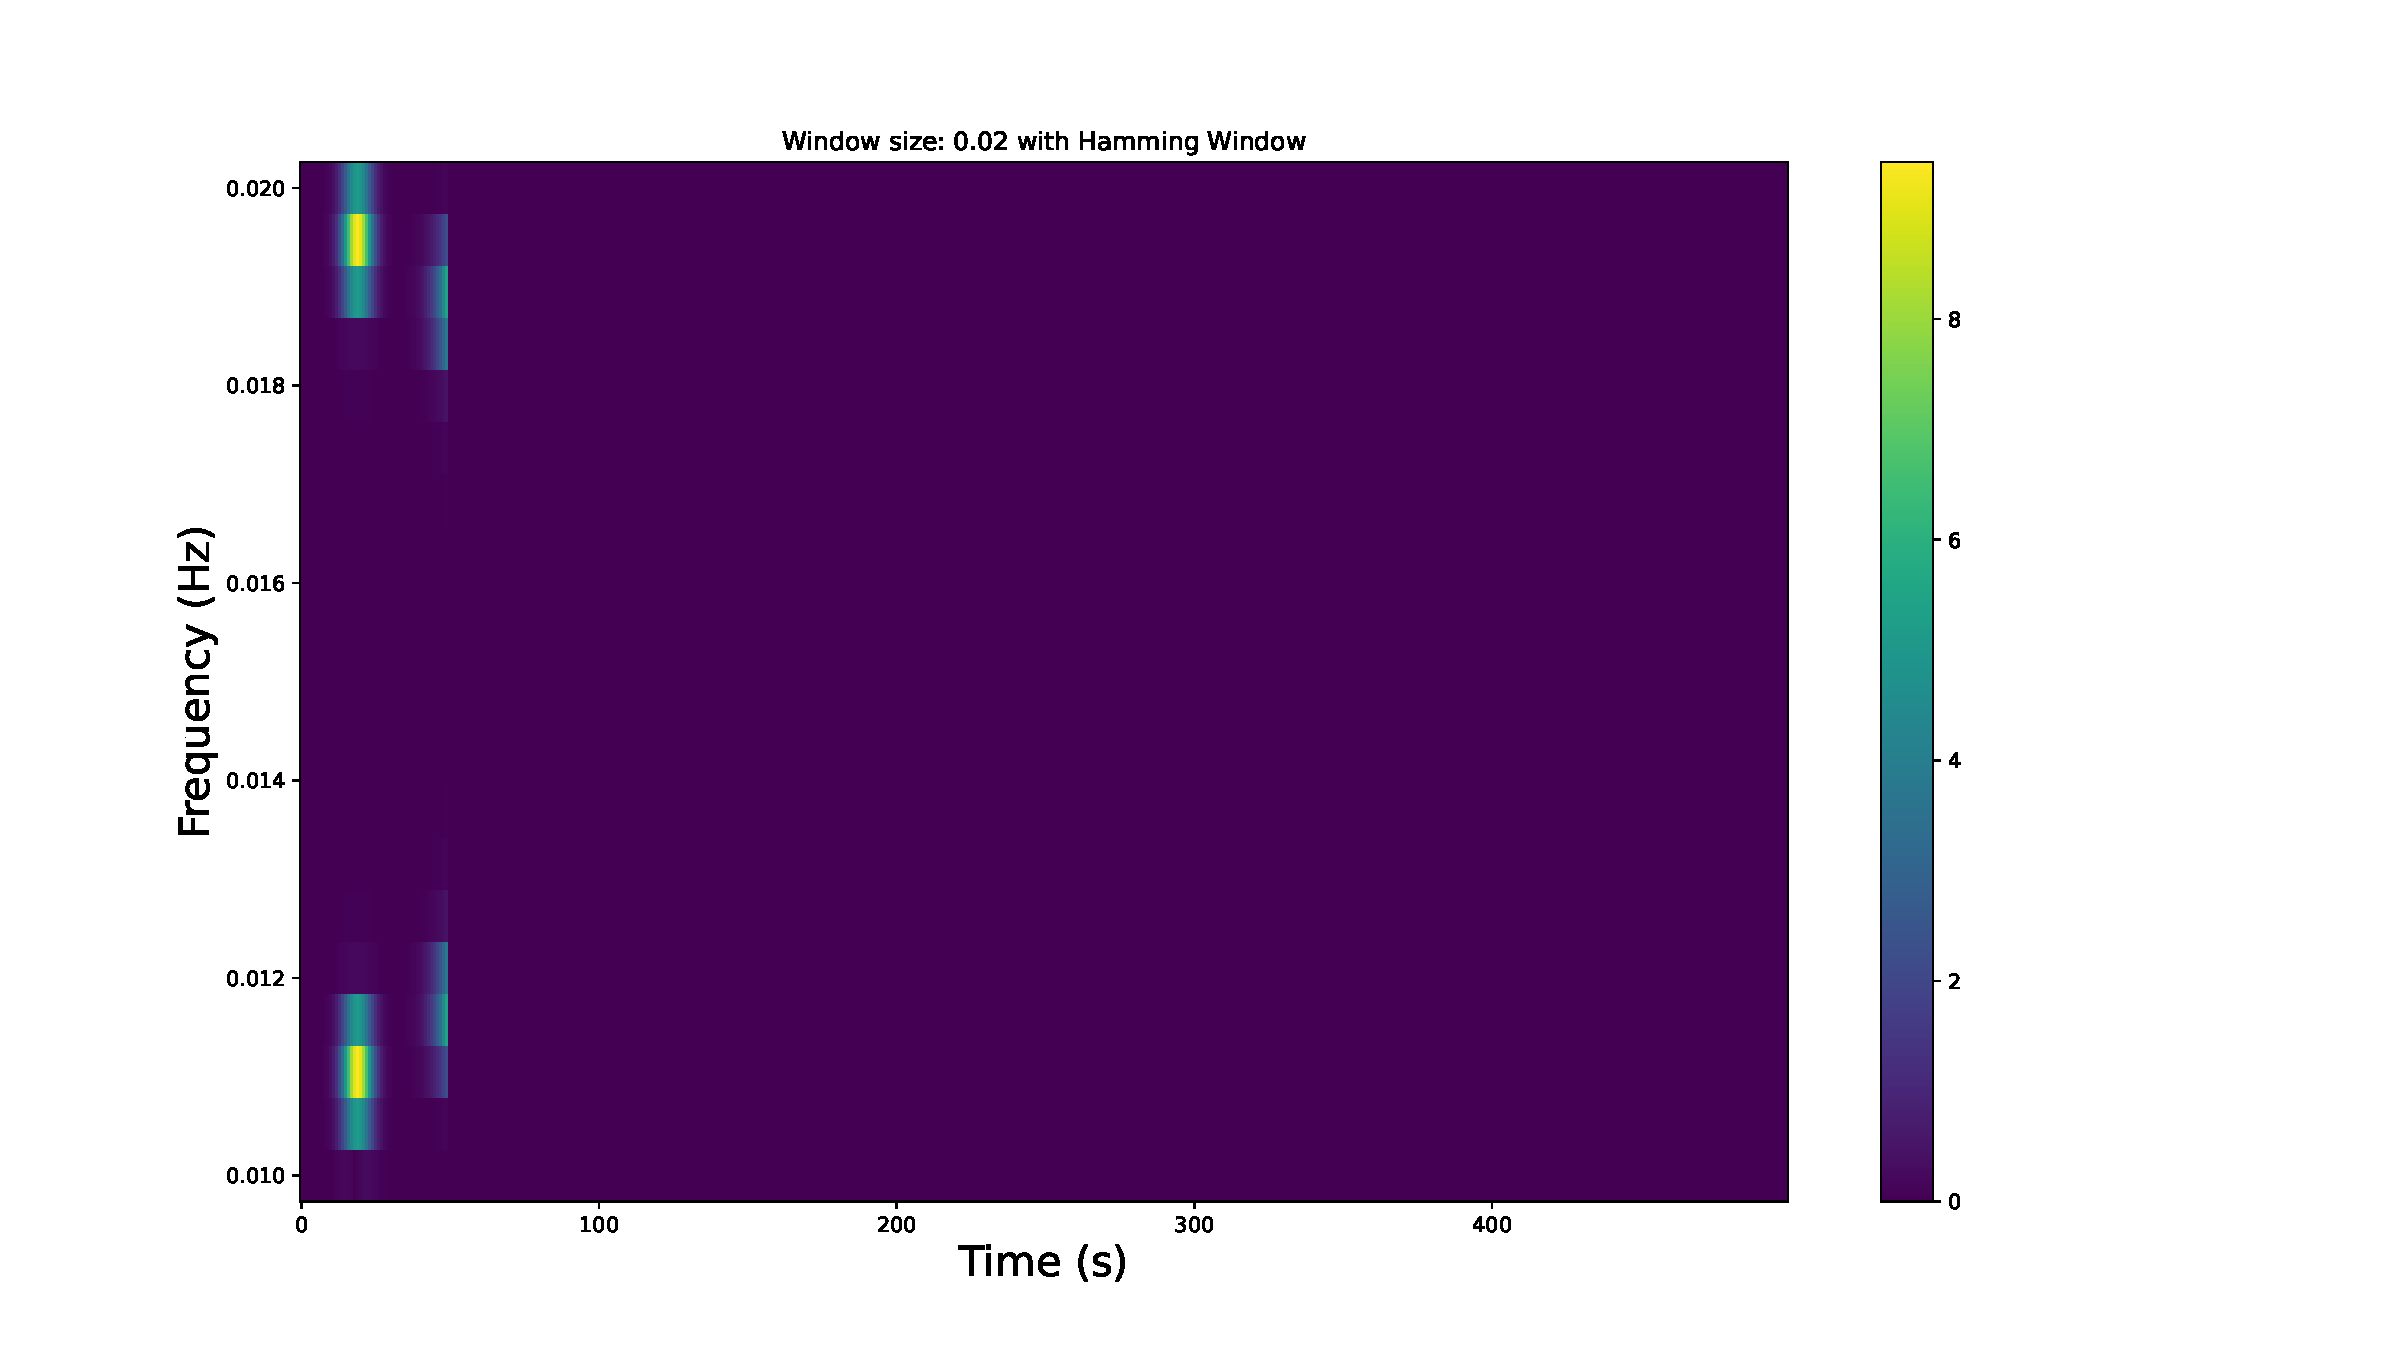
\includegraphics[width = \textwidth]{fig/2.d.1.pdf}
  \caption{Spektrogram med Hanning vindu}
  \label{fig: 2.d.1}
\end{figure}

\begin{figure}[h!]
  \centering
  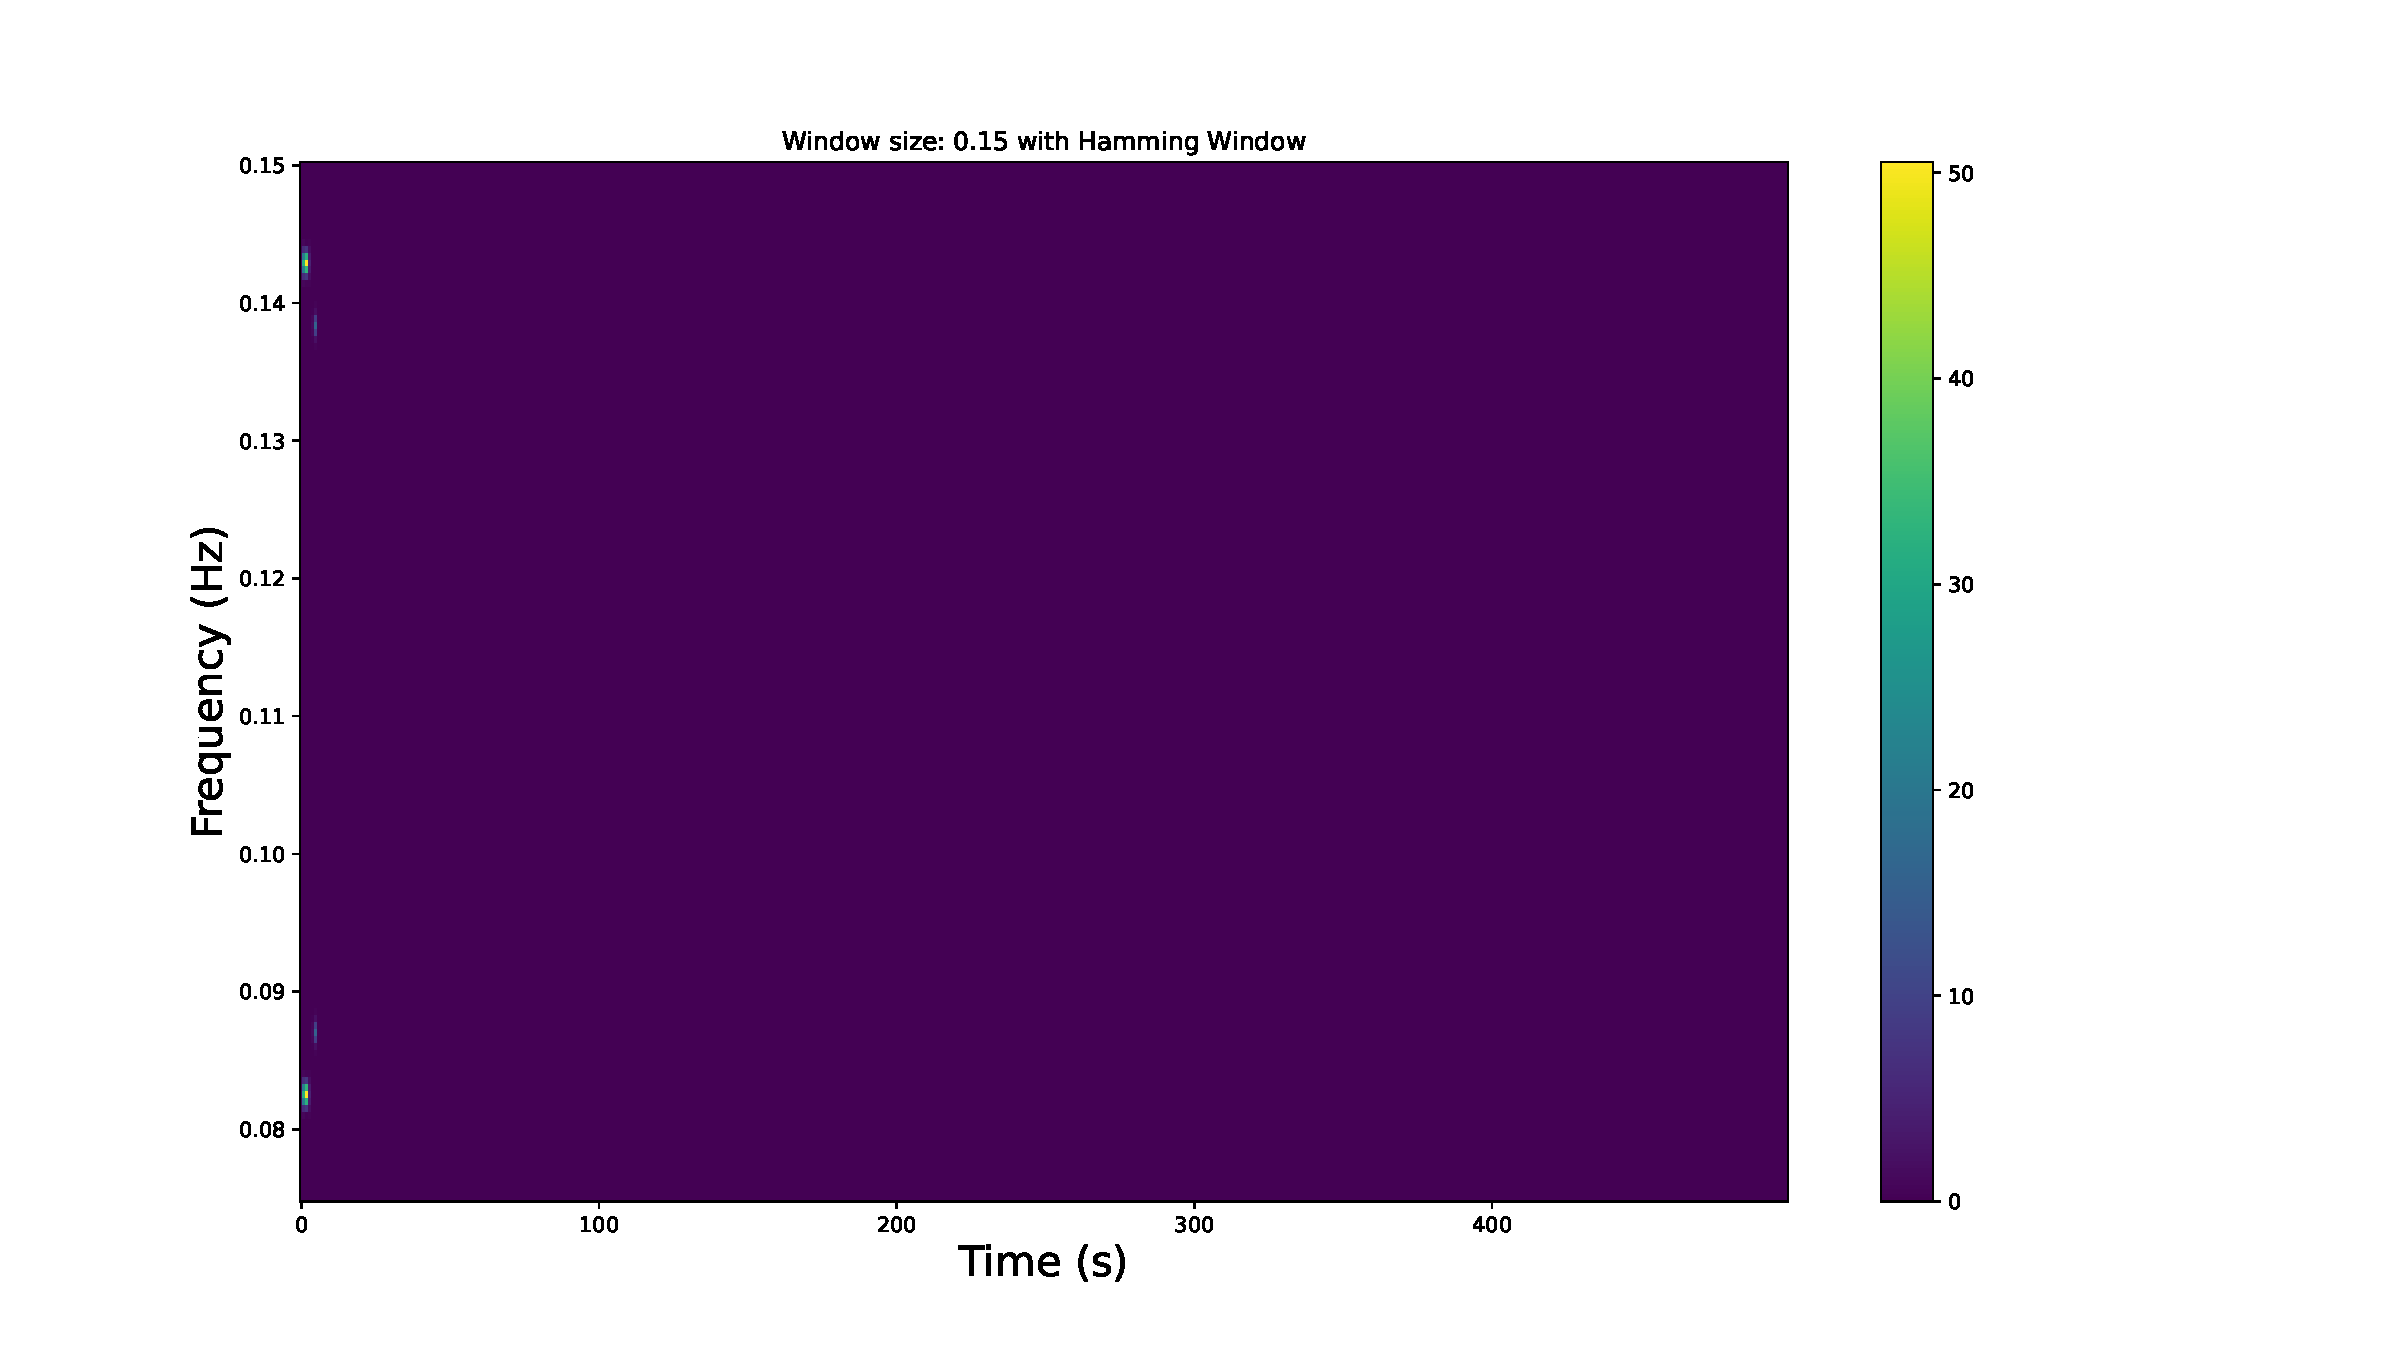
\includegraphics[width = \textwidth]{fig/2.d.2.pdf}
  \caption{Spektrogram med Hanning vindu}
  \label{fig: }
\end{figure}
Ettersom lydsignal i virkeligheten ikke har like brå slutt som når vi slicer de i STFT får vi mye mer realistiske resultat hvis vi smoother ut signalet ut med Hanningvinduet. 

\subsection*{e)}
\begin{figure}[h!]
  \centering
  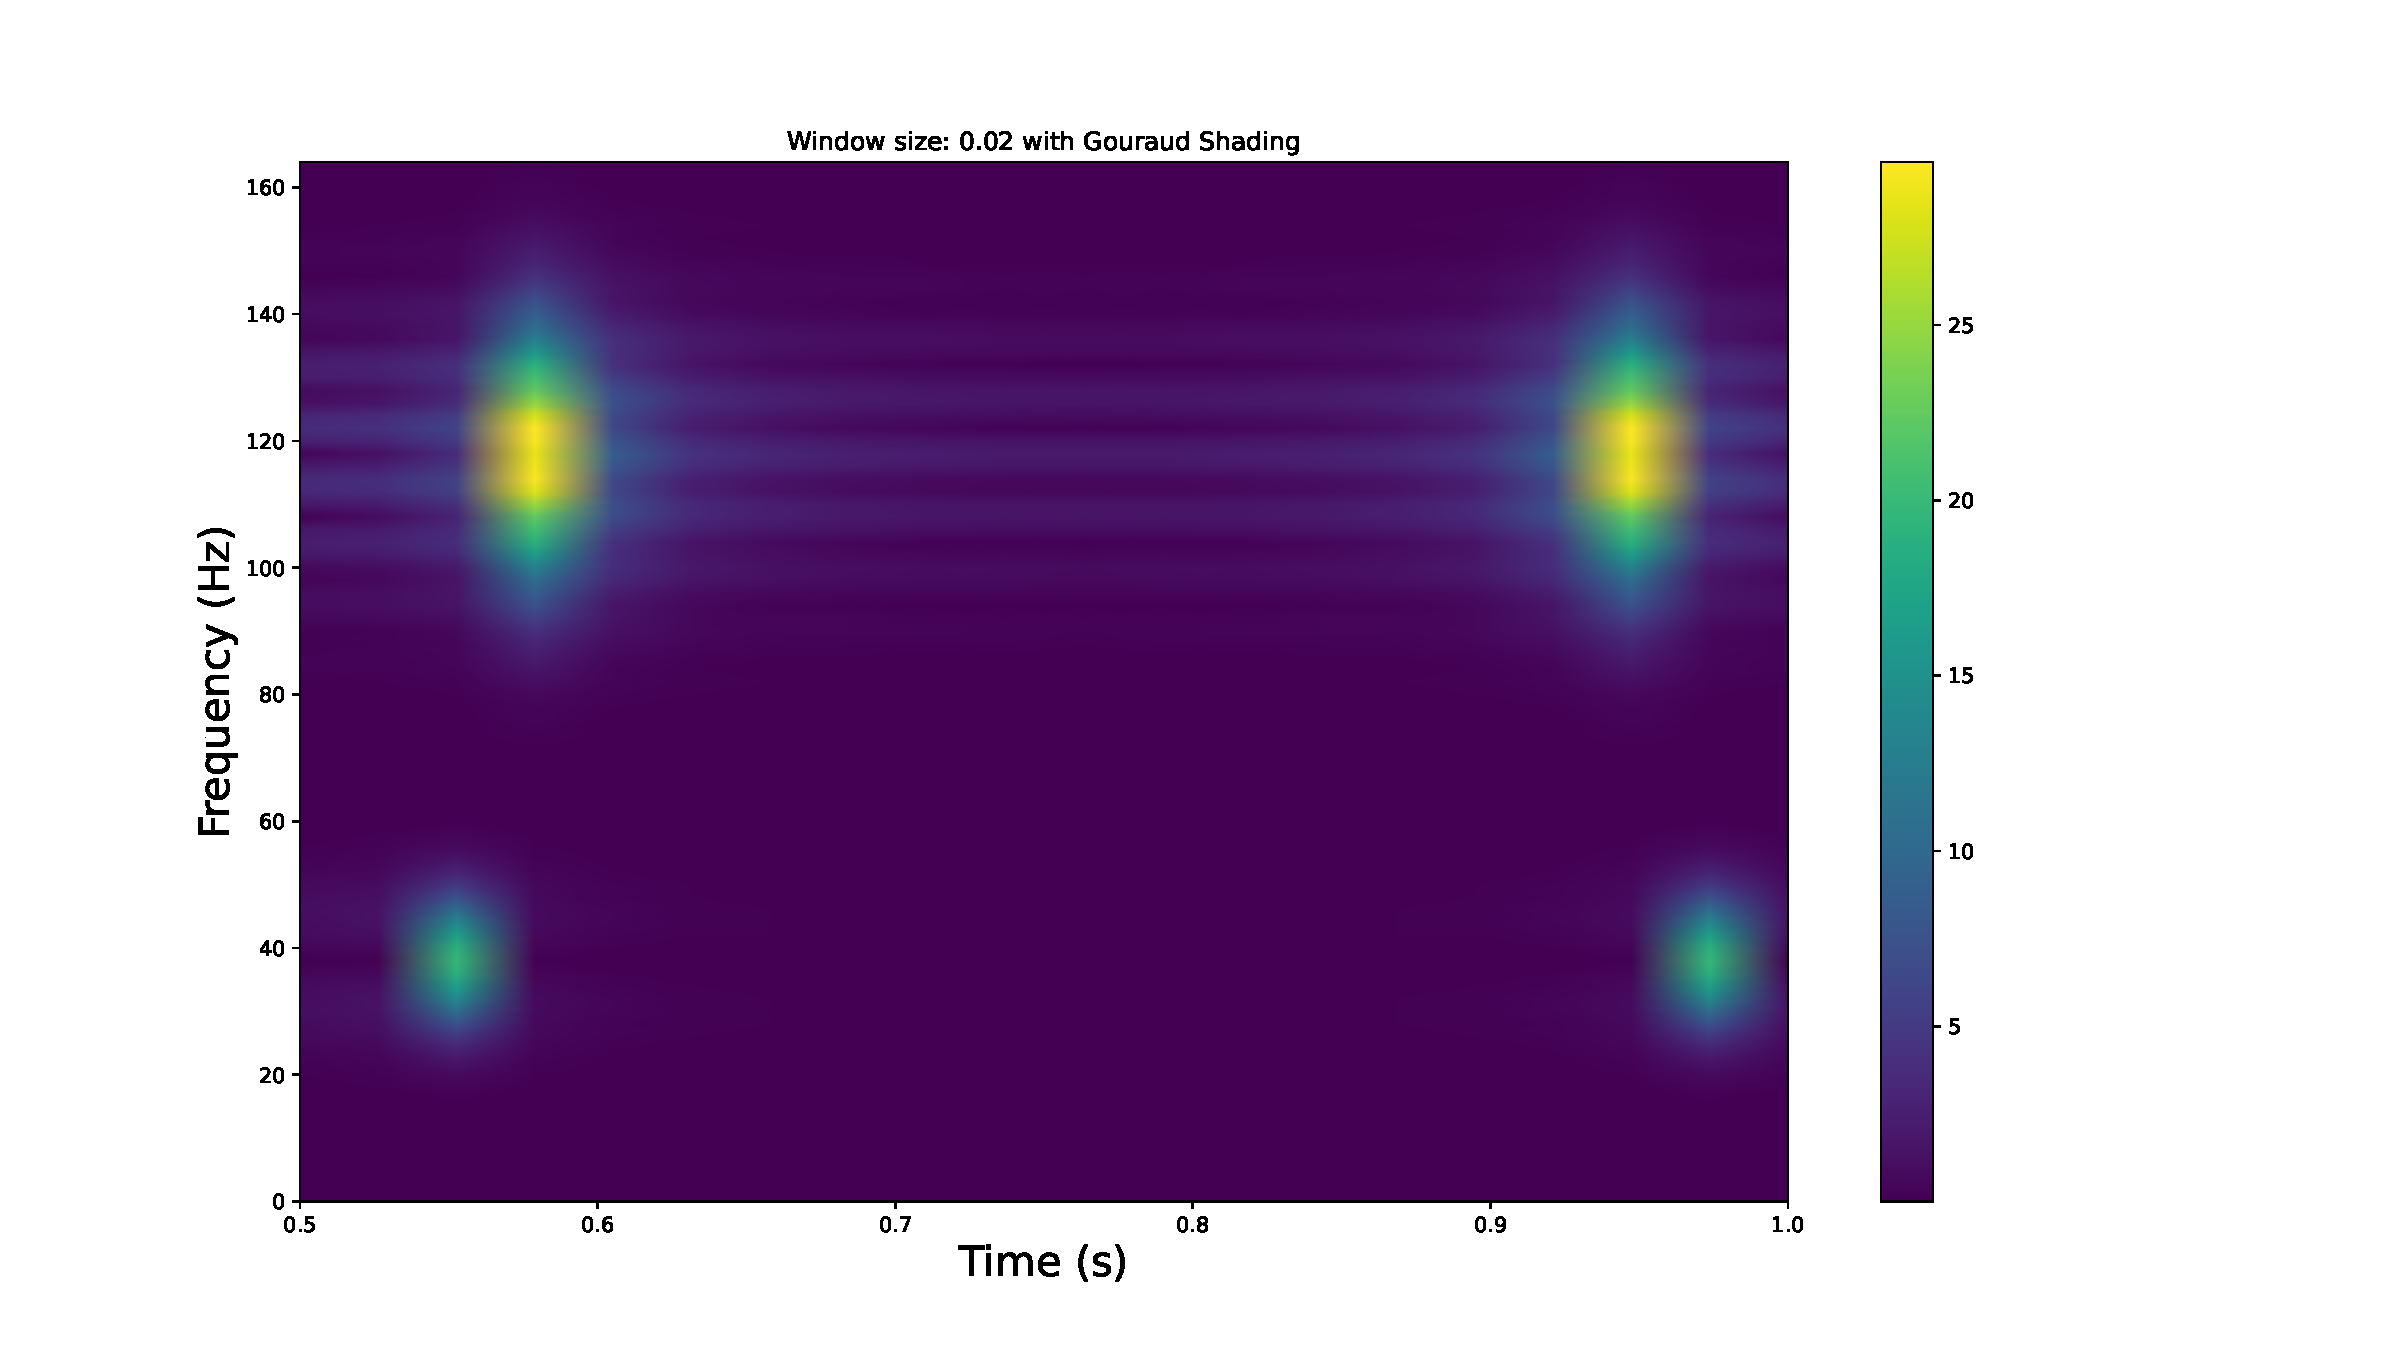
\includegraphics[width = \textwidth]{fig/2.e.1.pdf}
  \caption{}
  \label{fig: 2.e.1}
\end{figure}

\begin{figure}[h!]
  \centering
  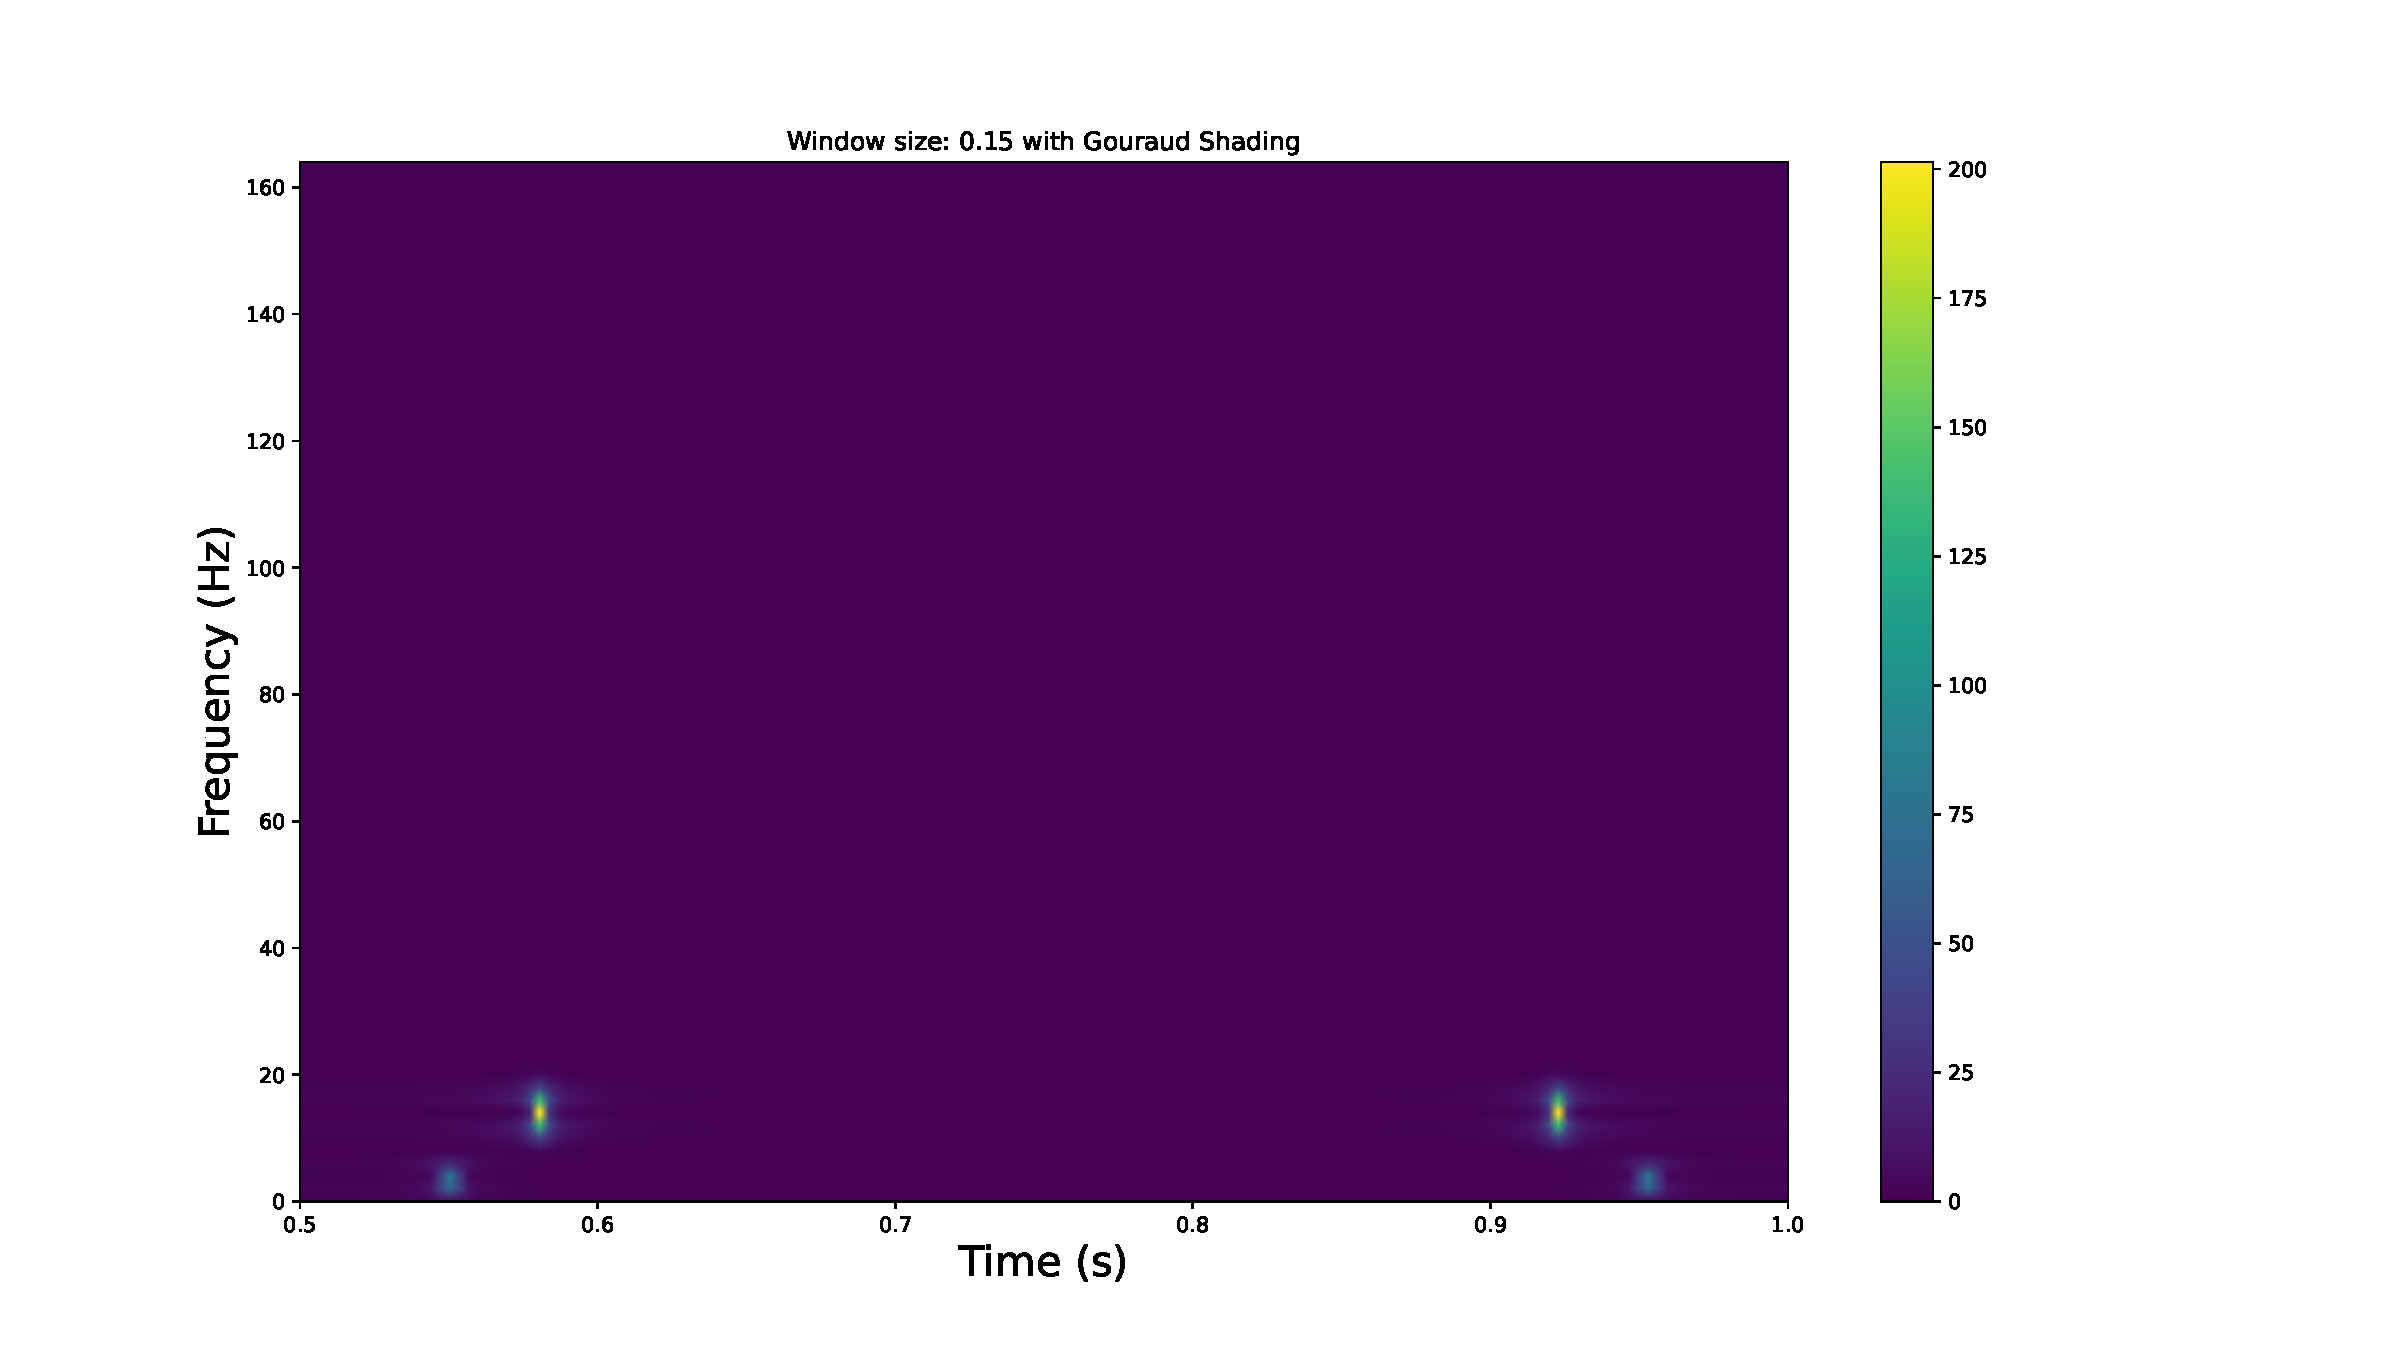
\includegraphics[width = \textwidth]{fig/2.e.2.pdf}
  \caption{Caption}
  \label{fig: 2.e.2}
\end{figure}

\newpage
\section*{Oppgave 3}
\subsection*{a)}
\begin{figure}[h!]
  \centering
  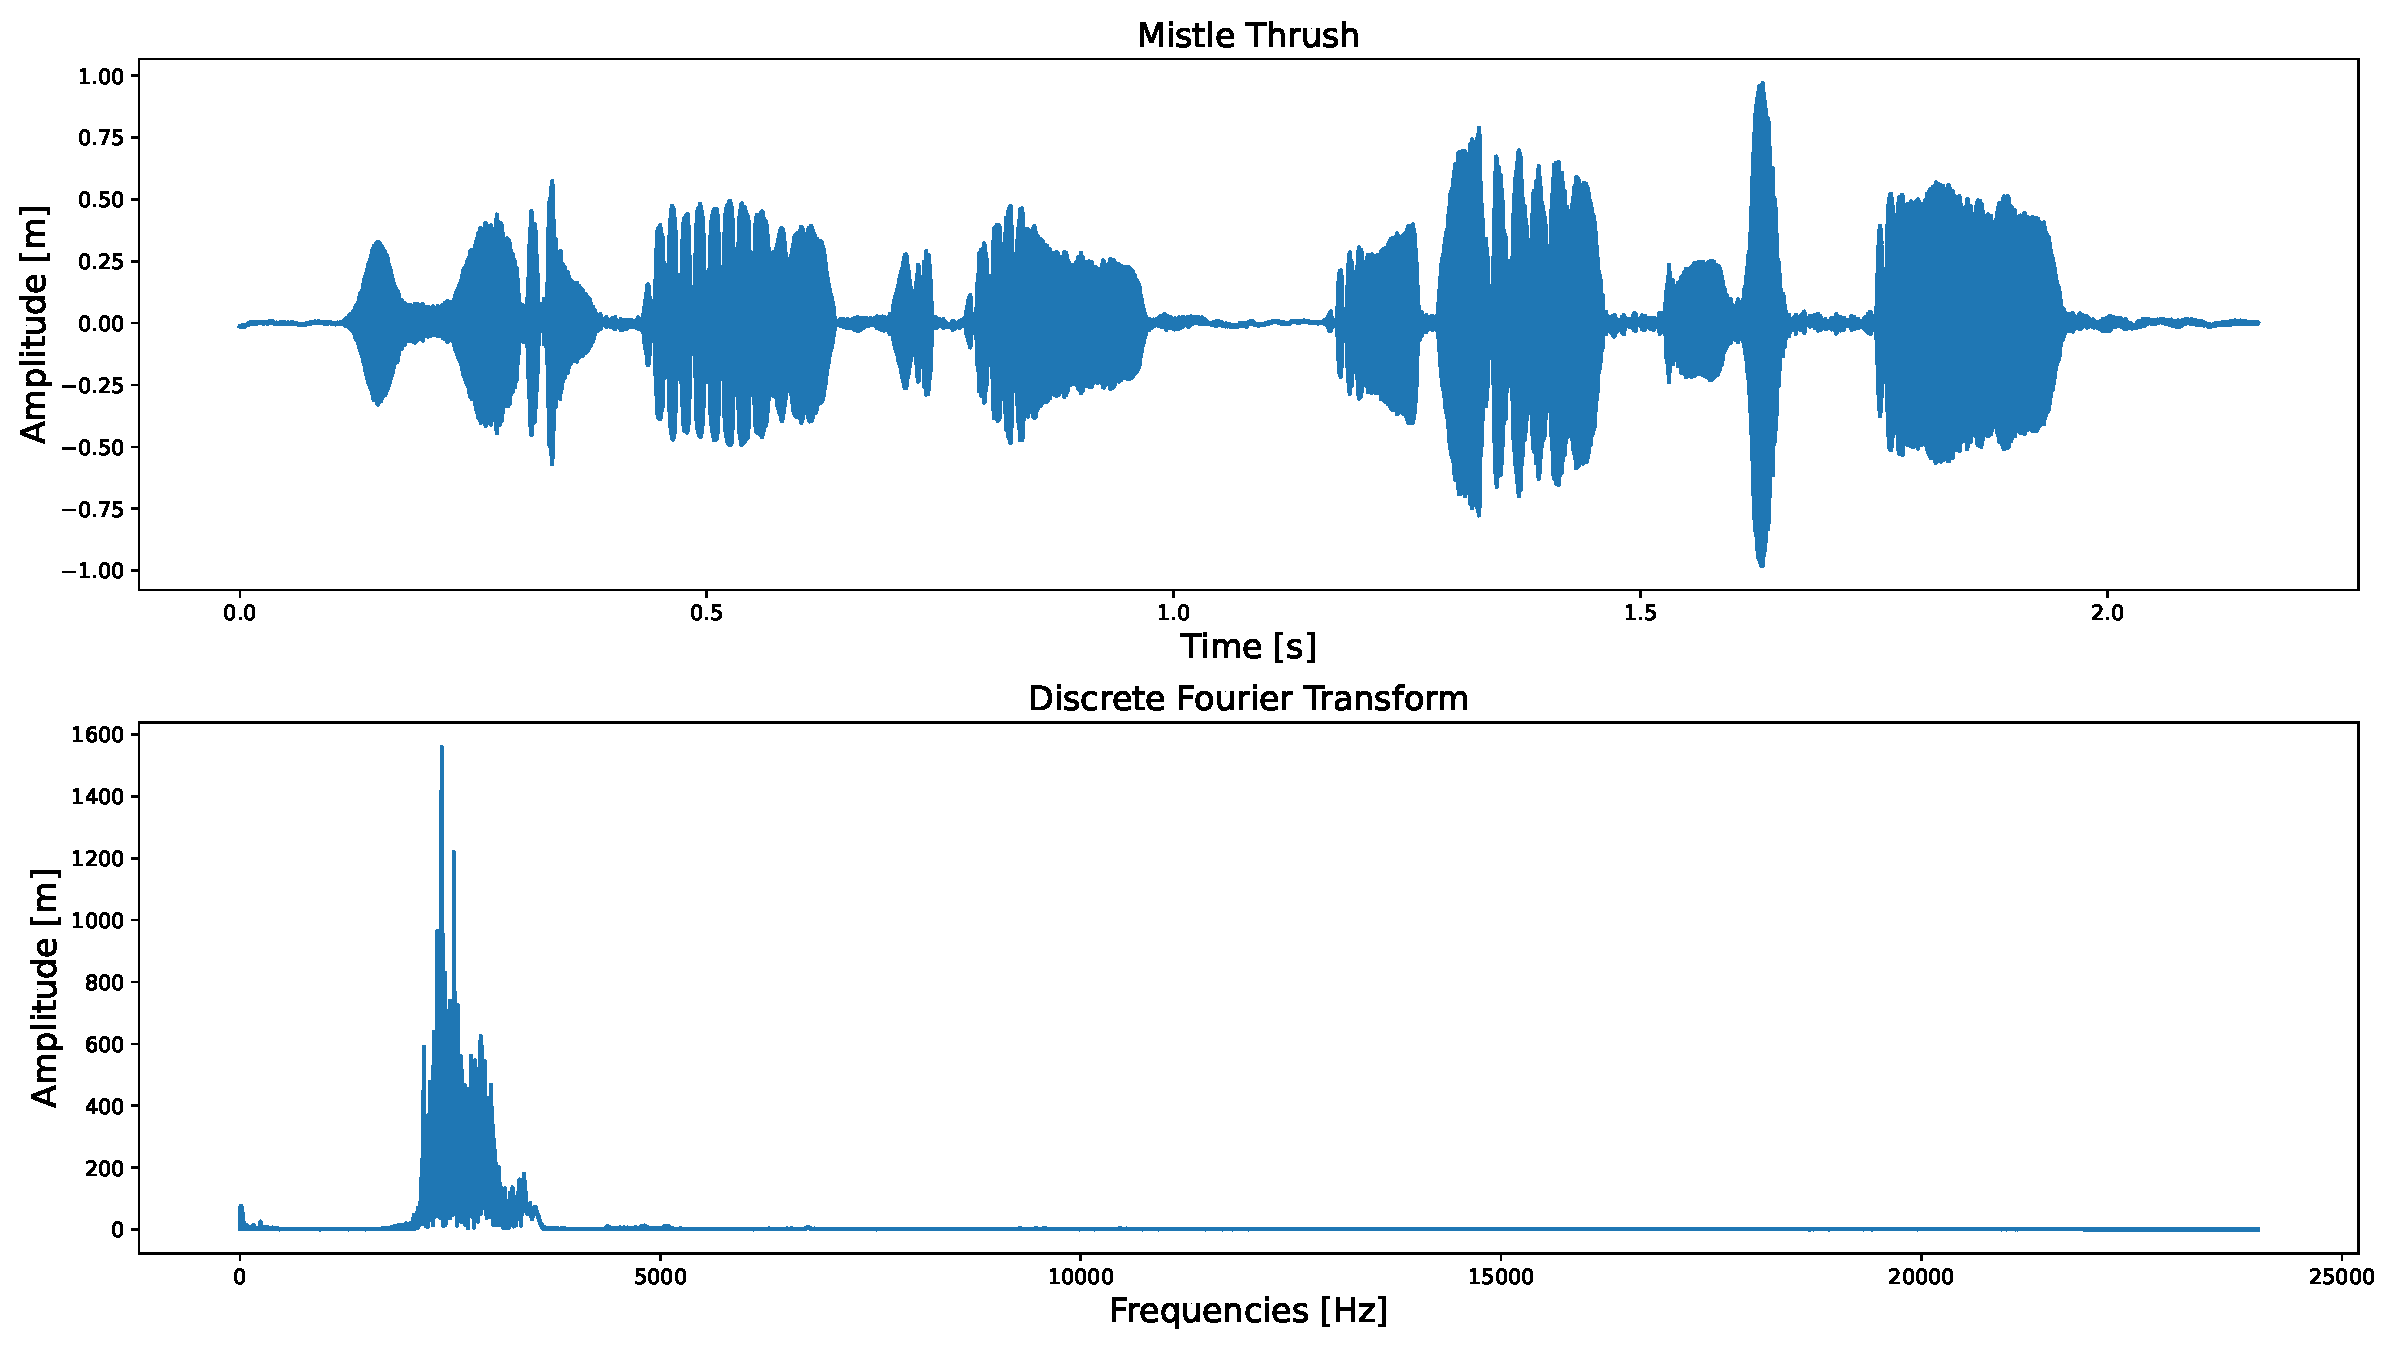
\includegraphics[width = \textwidth]{fig/3.a.pdf}
  \caption{Caption}
  \label{fig: 3.a}
\end{figure}
Det interessante frekvensområde ligger på ca 2.5 til 4 kHz. 
\subsection*{b)}
Sample frekvensen er på 48 kHz. Dette gir en Nyquist frekvens på 24 kHz. Ettersom mennesker bare hører opp til rundt 20 kHz har man dekket det hele potensielle behovet av frekvenser.

\subsection*{c)}

\subsection*{d)}




\end{document}